\begin{figure}[H]
    \centering
    \begin{adjustbox}{width=15cm,center}
      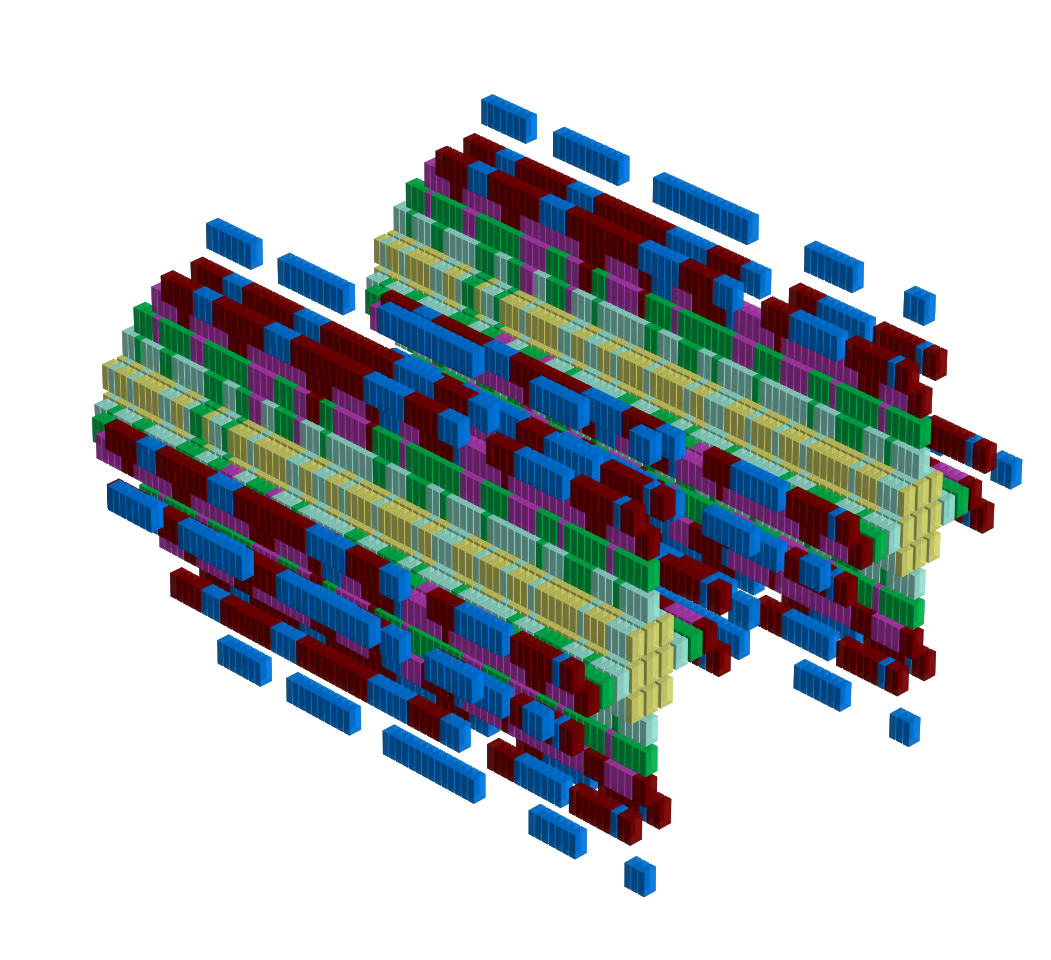
\includegraphics[width=10cm]{src/pulsespeed/pattern0-45.png}%
      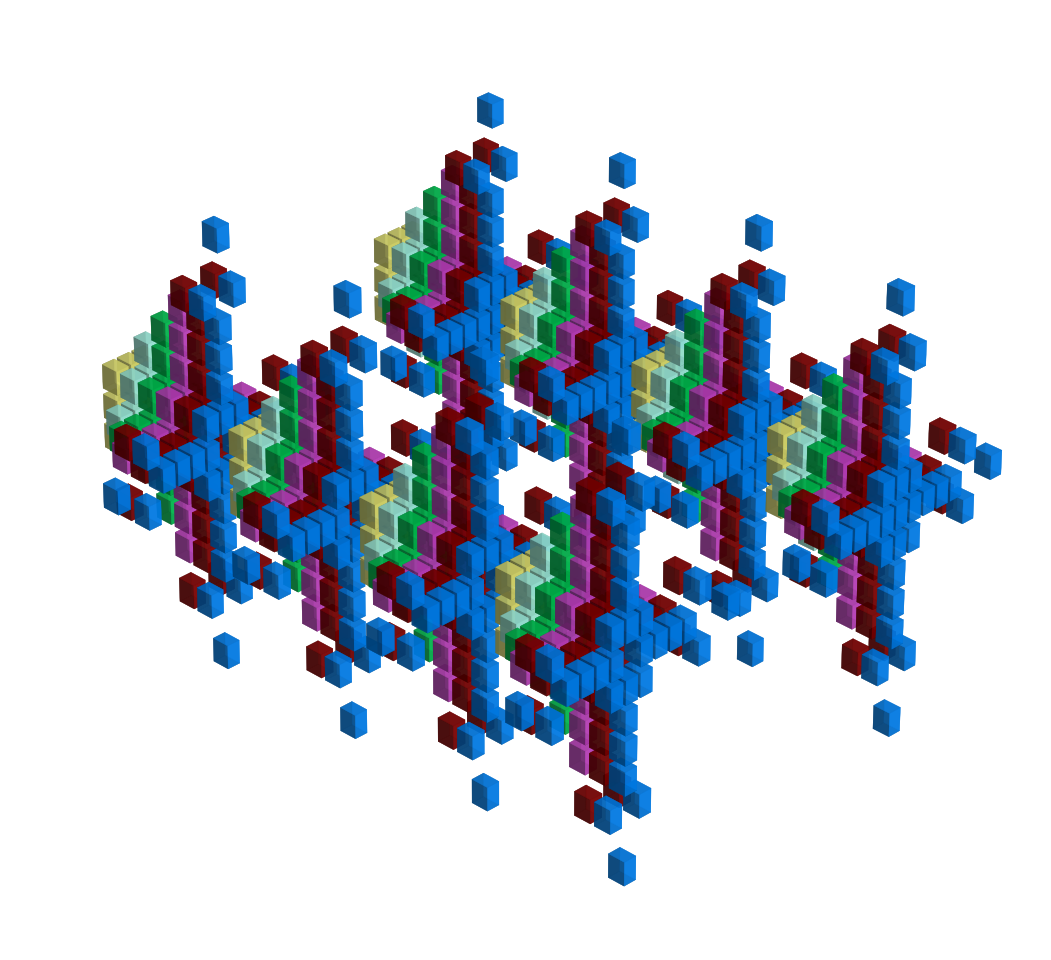
\includegraphics[width=10cm]{src/pulsespeed/pattern1-45.png}%
    \end{adjustbox}
    \caption{Effect of low and high values for Pulse Speed}
\end{figure}
\begin{figure}[H]
    \centering
    \begin{adjustbox}{width=15cm,center}
      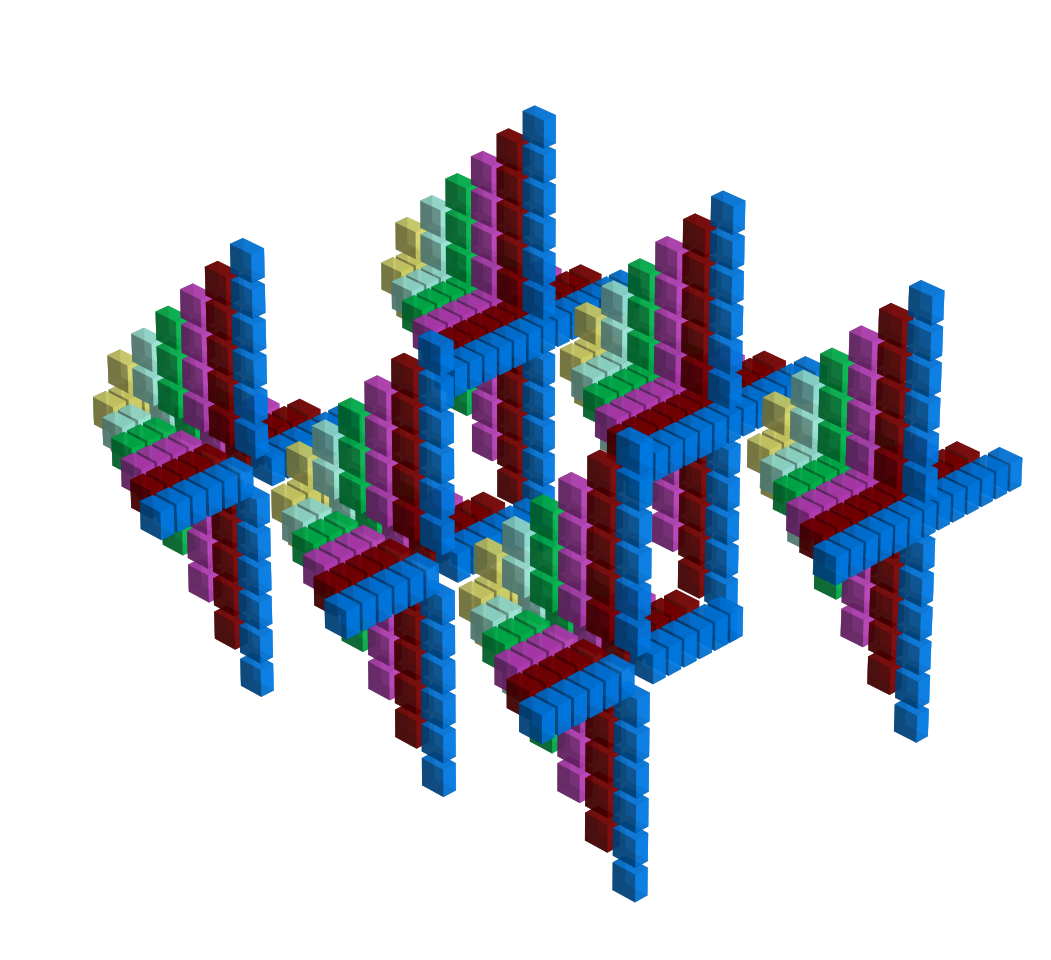
\includegraphics[width=10cm]{src/pulsewidth/pattern0-45.png}%
      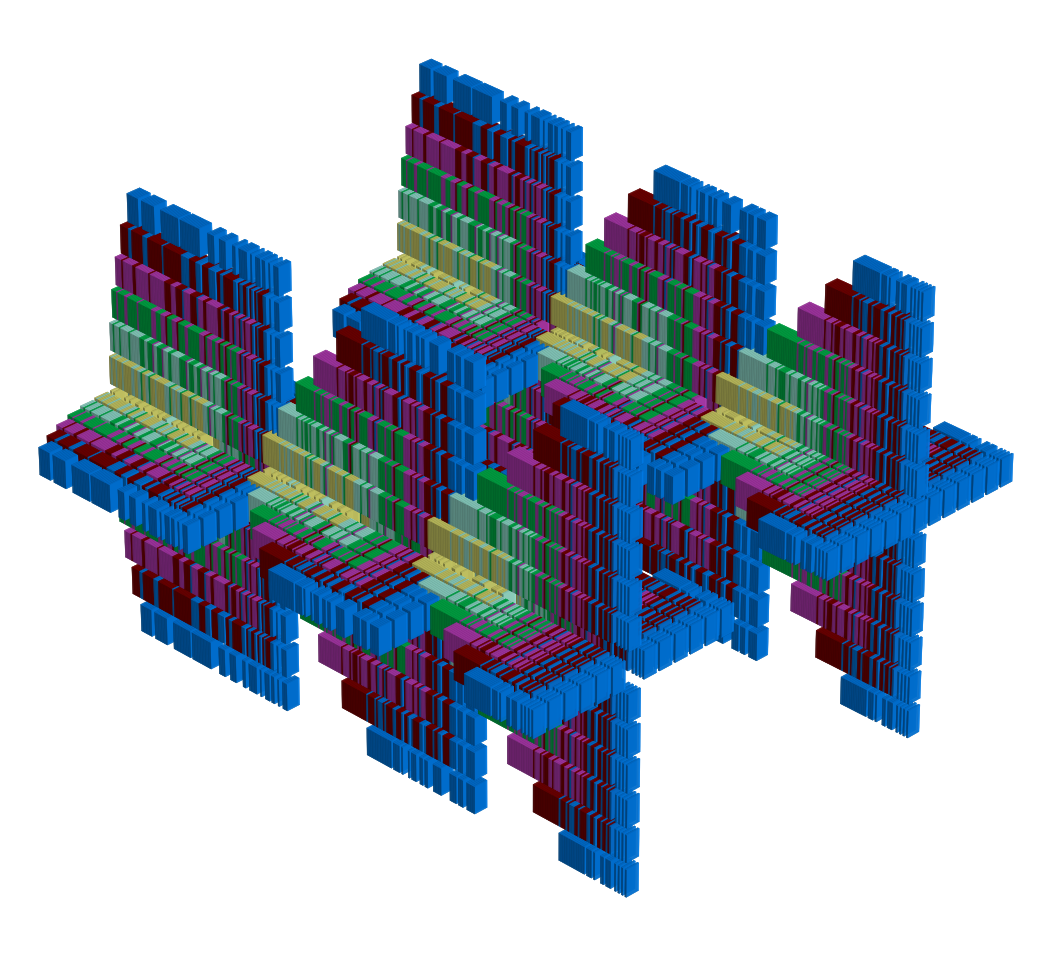
\includegraphics[width=10cm]{src/pulsewidth/pattern1-45.png}%
    \end{adjustbox}
    \caption{Effect of low and high values for Pulse Width}
\end{figure}
\clearpage
\section*{pulse speed/pulse width}
\label{sec:pulse_speed}
\lstset{style=6502Style}
\lstset{ 
   aboveskip=5pt,
   belowskip=0pt,
}

\begin{definition}[Jeffrey Says]
\setlength{\intextsep}{0pt}%
\setlength{\columnsep}{3pt}%
\begin{wrapfigure}{l}{0.12\textwidth}

\includegraphics[width=\linewidth]{src/callout/psych.png} 
\end{wrapfigure}
\small
\textbf{P to activate:} Usually if you hold down the button
you get a continuous stream. Setting the Pulse Speed allows you to
generate a pulsed stream, as if you were rapidly pressing and
releasing the FIRE button.
\\
\end{definition}


\begin{definition}[Jeffrey Says]
\setlength{\intextsep}{0pt}%
\setlength{\columnsep}{3pt}%
\begin{wrapfigure}{l}{0.12\textwidth}

\includegraphics[width=\linewidth]{src/callout/psych.png} 
\end{wrapfigure}
\small
\textbf{O to activate:} Sets the length of the pulses in a
pulsed stream output. Don’t worry about what that means - just get
in there and mess with it.
\\
\\
\end{definition}


\clearpage
\textbf{Lines 1189-1231. \icode{\textbf{MaybePPressed}}} 
\begin{lstlisting}[caption=From \icode{CheckKeyboardInput}.]
MaybePPressed   
  CMP #KEY_P ; P pressed
  BNE MaybeHPressed

  ; P pressed.
  LDA #$04
  STA currentVariableMode
  RTS 
\end{lstlisting}
\textbf{Lines 1189-1231. \icode{\textbf{UpdateVariableDisplay}}} 
\begin{lstlisting}[caption=From \icode{CheckKeyboardInputForActiveVariable}. Pressing the \icode{<} and > keys increments and
decrements the value in presetValueArray pointed to by \icode{X}\, i.e. \icode{currentVariableMode}.]
UpdateVariableDisplay   
        ...

        LDX currentVariableMode
        LDA lastKeyPressed
        CMP #KEY_GT ; > pressed?
        BNE MaybeLeftArrowPressed

RightArrowPressed
        ; > pressed, increase the value bar.
        INC presetValueArray,X
        LDA presetValueArray,X
        ; Make sure we don't exceed the max value.
        CMP maxValueForPresetValueArray,X
        BNE MaybeInColorMode
        DEC presetValueArray,X
        JMP MaybeInColorMode

MaybeLeftArrowPressed   
        CMP #KEY_LT ; < pressed?
        BNE MaybeInColorMode

        ; < pressed, decrease the value bar.
        DEC presetValueArray,X
        LDA presetValueArray,X
        ; Make sure we don't exceed the min value.
        CMP minValueForPresetValueArray,X
        BNE MaybeInColorMode
        INC presetValueArray,X
\end{lstlisting}
\clearpage

\textbf{Lines 1189-1231. \icode{\textbf{MaybePPressed}}:} When \icode{P} is pressed we don't
update a setting there and then as you might expect. Instead we get ready to display the 'Smoothing
Delay' control bar, by... loading the value \icode{\$04} to \icode{currentVariableMode}? Okay, we'll
go with that for now.

\textbf{Lines 1189-1231. \icode{\textbf{UpdateVariableDisplay}}:}  The next time we loop around
to \icode{Check\-KeyboardInput}, we hit this little piece of logic at the very top of it:

\begin{lstlisting}
CheckKeyboardInput   
        LDA currentVariableMode
        BEQ CheckForGeneralKeystrokes
        JMP CheckKeyboardInputForActiveVariable
\end{lstlisting}

Well, we just loaded \icode{\$01} to \icode{currentVariableMode} above so it's not zero.  It follows that
the \icode{BEQ} check will give a negative result (the check means 'is the value in \icode{A} equal to zero?'), 
so instead of forking to \icode{CheckForGeneralKeystrokes} we'll \icode{JMP} to \icode{CheckKeyboardInputForActiveVariable}.

This is where the function we're looking at here lives. As we can see the first thing it does is load 
\icode{currentVariableMode} to the \icode{X} register. This is because we're going to use it as an index
into an array we encountered in the previous chapter on Presets. This is the array \icode{presetValueArray}
which contains a lot of the settings we'll be looking at in this chapter huddled together like a gaggle
of ducklings, with \icode{pulseSpeed} near at index 4 (index 0 being taken by \icode{unusedPresetByte}):

\begin{lstlisting}
presetValueArray
unusedPresetByte        .BYTE $00
smoothingDelay          .BYTE $0C
cursorSpeed             .BYTE $02
bufferLength            .BYTE $1F
pulseSpeed              .BYTE $01 ; <-- Index $04
...
\end{lstlisting}

With \icode{X} set to 4 we can now use it increment the value for \icode{pulseSpeed} by
simply executing:
\begin{lstlisting}
        INC presetValueArray,X
\end{lstlisting}
And decrement it by doing:
\begin{lstlisting}
        DEC presetValueArray,X
\end{lstlisting}
This is handy, and worth remembering as the technique will be reused for adjusting other values that 
we look at that also live in \icode{presetValueArray}.

\clearpage

\clearpage
\begin{lstlisting}[caption=From \icode{MainInterruptHandler}.]
;-------------------------------------------------------
; MainInterruptHandler
;-------------------------------------------------------
MainInterruptHandler
        ...
        ; Player has pressed fire.
PlayerHasPressedFire   
        LDA stepsExceeded255
        BEQ DecrementPulseWidthCounter
        LDA stepsSincePressedFire
        BEQ IncrementStepsSincePressedFire
        JMP DrawCursorAndReturnFromInterrupt

IncrementStepsSincePressedFire   
        INC stepsSincePressedFire

DecrementPulseWidthCounter   
        LDA currentPulseWidth
        BEQ DecrementPulseSpeedCounter
        DEC currentPulseWidth
        BEQ DecrementPulseSpeedCounter
        JMP UpdatePixelBuffersForPattern

DecrementPulseSpeedCounter   
        DEC currentPulseSpeedCounter
        BEQ RefreshPulseSpeed
        JMP DrawCursorAndReturnFromInterrupt

RefreshPulseSpeed   
        LDA pulseSpeed
        STA currentPulseSpeedCounter
        LDA pulseWidth
        STA currentPulseWidth

        ; Finally, update the pixel buffers with a byte
        ; each for the current pattern.        
UpdatePixelBuffersForPattern    
        INC currentStepCount
        LDA currentStepCount
        CMP bufferLength
        BNE UpdateBaseLevelArray

        LDA #$00
        STA currentStepCount
\end{lstlisting}
\clearpage

\textbf{Lines 1189-1231. \icode{\textbf{MainInterruptHandler}}:} 
As you may remember the \icode{MainInterruptHandler} runs every 1/60th of a
second.  You may also recall its main job is to fill the pixel buffers (e.g.
pixelXPositionArray, pixelYPositionArray and so on) so that the MainPaintLoop
can use them to paint the screen. 

\textbf{Lines 1189-1231. \icode{\textbf{CheckIfTrackingActivated}}:} 
\icode{trackingActivated} comes into play here. The idea is that if 'tracking'
is enabled then we should do a re-paint of the last entry in the buffers that was
processed by \icode{MainPaintLoop}. Naturally, if a pixel is being painted twice
over this will create a 'tracking' effect, as though the pattern is trailing a 
glowing tail after it.

We use the value in \icode{trackingActivated} to decide whether or not to paint
the previously processed position in the buffers by simply \icode{AND}'ing the
two together.

\begin{lstlisting}
        LDA previousIndexToPixelBuffers
        AND trackingActivated
        BEQ DrawCursorAndReturnFromInterrupt
\end{lstlisting}

If it's zero, we bail out
completely until the next interrupt by jumping to \icode{DrawCursor\-AndReturnFromInterrupt}.
But if we get a non-zero value that means tracking is enabled and 
we should go ahead and refresh the values in the buffers at the index given
by the value in \icode{previousIndex\-ToPixelBuffers}. So we 'fall through' instead to
\icode{UpdatePositionArrays} and a number of other sub-routines that update the
values of the previous position in our pixel buffers.
\clearpage

